\documentclass[11pt]{article}
% -*-coding: iso-latin-1  -*-
\usepackage{graphicx}
\usepackage{url}
\usepackage{hyperref}
\usepackage{wrapfig}
\usepackage{mathtools}




% source code
\usepackage{color}
\usepackage{xcolor}
\usepackage{listings}
\lstset{language=tex}

\usepackage{caption}
\DeclareCaptionFont{white}{\color{white}}
\DeclareCaptionFormat{listing}{\colorbox{gray}{\parbox{\textwidth}{#1#2#3}}}
\captionsetup[lstlisting]{format=listing,labelfont=white,textfont=white}


\usepackage[spanish, english]{babel}
\usepackage[utf8]{inputenc}

%This is for removing coloured boxes around the links and internal references. I don't like those boxes%
\hypersetup{
    colorlinks=false,
    pdfborder={0 0 0},
}


\title{\textbf{\underline{Case Studies I}}}
\author{
        Jose Alberto Navas Guerrero (Janague)\\
       Master's Official Software Libre\\
       Professor: Gregorio Robles\\
	Universidad Rey Juan Carlos\\
        Spain
}

\begin{document}
\maketitle

\begin{abstract}
 This report is a summary of the lectures of case studies I about \LaTeX , MariaDB, GNU R, translation in Libre software, unix shells, and free software hypervisors.  
\end{abstract}


\begin{center}
\textsc CC BY-SA 3.0\\[0.2cm]

\includegraphics[scale=0.5]{img/by-sa} \\ % Include license
{\small http://creativecommons.org/licenses/by-sa/3.0}\\

\end{center}
\newpage

\tableofcontents

% \listoffigures

\newpage

\section{Introduction}

This report analyzes the used outstanding free software products and techniques, in particular \LaTeX, MariaDB (the original product was MySQL, but I find interesting to analyze a folk of free software product), GNU R statistical product,  translation, unix shell, and hypervisors. 

  


%------------------------------------------------------------------------------
% 1. LaTex
\section{\LaTeX}

\subsection{Introduction}
\TeX\  is a high-quality typesetting system, which was written by Donald Knuth of Stanford University, it includes features designed for the production of technical and scientific documentation. \LaTeX\  is the de facto standard for the communication and publication of scientific documents. LaTeX is one of the first software available as free software (LaTeX Project Public License). \TeX is Free software (“public domain” dedication) but any modified version must not be called \TeX\ .

\textbf{Donald Knuth} started to develop TeX during a sabbatical year, in \textbf{1978}. \TeX is an electronic typography system commonly used for producing high-quality documents. From the start, Knuth used a licence that today would be considered a free software licence. When the system was considered sufficiently stable, in 1985, he maintained that licence. At that time, TeX was on the largest and most well-known systems that could be considered free software.

\TeX\ is the basic typesetting engine, \LaTeX\ is a large set of macros, which are maintained by an international group of experts.

\subsection{\TeX/\LaTeX\ history and an intro to TeX files}
In 1978, Donald Knuth started developing \TeX while revising the second volume of his "Art of Computer Programming", because he did not find properly technology to make that.

Another important actor was Leslie Lamport that developed \LaTeX to make it easier for people to use, using it indirectly way, \LaTeX\ uses the \TeX\ typesetting program and writer types simple commands and \LaTeX does the work for us. In summary, \LaTeX\ is a practical improvement on \TeX, and the current stable version of \LaTeX, called \LaTeX2e.

\subsection{What is (La) \TeX\ }
\subsubsection{\TeX\ }
\TeX\ is a low-level markup and programming language and interpreter created by \emph{Donald Knuth} in 1977 to typeset documents attractively and consistently to digital printing. The historical context was that Donald Knuth did not like the style of type in 1st edition, and then he decided to prepare a 2nd edition of Volume 2 implementing and writing in \TeX. After that all volumes used \TeX. 

The two main aims:
\begin{itemize}
  \item Highest quality
  \item Highest durability
\end{itemize}

With the release of 8-bit character support in 1989, \TeX\ development has been essentially frozen with only bug fixes released periodically. The version numbers of \TeX\ are converging toward $\pi$ , with a current version number of 3.1415926, and the design was frozen in October 1990. He firmly believes that having an unchanged system that will produce the\emph{ same output now and in the future} is more important than introducing new features.

The name \TeX\  derives from the Ancient Greek word $\tau\varepsilon\chi\nu\eta$ /tejné/, that means skill, art, and technique. 


The usage is popular in academia, especially in mathematics, computer sciences, engineering, and physics.

\TeX can use about 300 low-level primitives, but these are rarely used directly users, who usually uses \LaTeX\ . 

In relation to \TeX\ Knuth created MetaFont too, although it is not really part of \TeX , the implementation of Knuth uses it. Metafont is a font description language to describe characters (glyphs) algorithmically with geometrical equations, in which it uses Bézier curve. Currently, Adobe PostScript fonts may be used instead. And its version is number $e$.
 
\subsubsection{\LaTeX\ }
LaTeX (pronounced either "Lah-tech" or "Lay-tech") is a set of macros based on \TeX primitives created by Leslie Lamport. Its purpose is to simplify \TeX typesetting, especially for documents containing mathematical formulae. Within the typesetting system, its name is formatted as \LaTeX\. The first release in 1985 and current version is 2e. \LaTeX\ is written in  \TeX.

Since \LaTeX\  comprises a group of \TeX commands and incorporates document styles for books, letters, slides, etc. \LaTeX\  document processing is essentially programming. You create a text file in \LaTeX\  markup, which \LaTeX\ reads to produce the final document.

Its license is free software, in particular, \LaTeX\ Project Public License, which is OSI-compliant and no-copyleft. 

The \LaTeX\ -like approach can be called WYSIWYM ("What You See Is What You Mean"), in contrast to WYSIWYG ("What You See Is What You Get")


\subsubsection{Advantages and caveats }
\begin{itemize}
    \item Flexibility and Scalability: Document sources can be read with any text editor and understood, unlike the complex binary and XML formats used with WYSIWYG programs.
    \item Control: You can concentrate purely on the structure and contents of the document, not get caught up with superficial layout issues.
    \item Stability and Quality: You don't need to manually adjust fonts, text sizes, line heights, or text flow for readability, as LaTeX takes care of them automatically.
    \item Portability: In \LaTeX\  the document structure is visible to the user, and can be easily copied to another document. In WYSIWYG applications it is often not obvious how a certain formatting was produced, and it might be impossible to copy it directly for use in another document.
    \item Scalability and Stability: The layout, fonts, tables and so on are consistent throughout the document.
    \item Flexibility, Quality and Scalability: Mathematical formulae can be easily typeset with high quality output.
    \item Control and Scalability: Indexes, footnotes, citations and references are generated easily.
    \item Flexibility and portability: Since the document source is plain text, tables, figures, equations, etc. can be generated programmatically with any language.
    \item Quality: You are forced to structure your documents correctly.
    \item Portability: Accurate and precise output in any device.
    \item Control, quality and scalability: Preventing formatting errors since \LaTeX\ forces to declare logical structure.
    \item Control: Separating content and styling.
    \item Portability: Easy to make global changes and encourage content reuse.
\end{itemize}

On the other hand, the caveats are
\begin{itemize}
    \item Hard learning curve.
    \item You generally need to know the necessary commands for \LaTeX\  markup.
    \item Design of a whole new layout is difficult and takes a lot of time.
    \item You don't (usually) see the final version of the document when editing it.
    \item It can sometimes be difficult to obtain a certain look for the document.
\end{itemize}

\subsubsection{MS Word vs \LaTeX\ }
\textbf{Compare kerning}

Kerning is the process of selectively adjusting the spacing between letters pairs to improve the overall appearance of text. 

\begin{table}[ht]
\centering
\begin{tabular}{cc}
MS Word Kerning & \LaTeX\ Kerning \\

\includegraphics[scale=1]{img/kerning_word}&
\includegraphics[scale=1]{img/kerning_latex}\\
\end{tabular}
\label{tab:gt}
\caption{Compare kerning}
\end{table}

\textbf{Compare Small Caps}

Most word processors create fake small capitals by adjusting the size of capitals.

\begin{table}[ht]
\centering
\begin{tabular}{cc}
MS Word Small Caps & \LaTeX\ Small Caps \\

\includegraphics[scale=0.6]{img/sc_word}&
\includegraphics[scale=0.6]{img/sc_latex}\\
\end{tabular}
\label{tab:gt}
\caption{Compare Small Caps}
\end{table}

\textbf{Ligatures}

A good typesetting programmer should always use contextual intelligence and substitution tables to determine whether ligatures are needed. 

\begin{table}[ht]
\centering
\begin{tabular}{cc}
MS Word Ligatures & \LaTeX\ Ligatures \\

\includegraphics[scale=0.6]{img/ligatures_word}&
\includegraphics[scale=0.6]{img/ligatures_latex}\\
\end{tabular}
\label{tab:gt}
\caption{Compare Ligatures}
\end{table}

\subsubsection{Installing \LaTeX\ }
To installing in Debian the command is

\begin{lstlisting}
$sudo apt-get install 	texlive-latex-base \
			texlive-latex-extra \
			texlive-latex-recommended
\end{lstlisting}

For edition a text editor is enough. In the \LaTeX\ distribution there are program for processing your \LaTeX\ source files into PDF or DVI documents. Finally, a PDF/DVI viewer for previewing and printing documents.

\subsubsection{Creating a basic document }

The simplest document (source code) in file called helloWorld.tex
\begin{lstlisting}
	% Hello world program in LaTeX
	\documentclass{article}

	\begin{document} 
		Hello world! This is a minimal \LaTeX{} document
	\end{document}
\end{lstlisting}

The output

	Hello world! This is a minimal \LaTeX{} document

The document workflow is the following:

\begin{lstlisting}
janague@gon:~/Documents/mswl/mswl_csi/doc/example$ latex 
helloWorld.tex 
This is pdfTeX, Version 3.1415926-usepackage{color}
\usepackage{xcolor}
\usepackage{listings}

\usepackage{caption}
\DeclareCaptionFont{white}{\color{white}}
\DeclareCaptionFormat{listing}{\colorbox{gray}{\parbox{\textwidth}
{#1#2#3}}}
\captionsetup[lstlisting]{format=listing,labelfont=white,
textfont=white}2.5-1.40.14 (TeX Live 2013/Debian)
 restricted \write18 enabled.
entering extended mode
(./helloWorld.tex
LaTeX2e <2011/06/27>
Babel <3.9f> and hyphenation patterns for 13 languages loaded.
(/usr/share/texlive/texmf-dist/tex/latex/base/article.cls
Document Class: article 2007/10/19 v1.4h Standard LaTeX document 
class
(/usr/share/texlive/texmf-dist/tex/latex/base/size10.clo))
No file helloWorld.aux.
[1] (./helloWorld.aux) )
Output written on helloWorld.dvi (1 page, 344 bytes).
Transcript written on helloWorld.log.
janague@gon:~/Documents/mswl/mswl_csi/doc/example$ ls
helloWorld.aux  helloWorld.dvi  helloWorld.log  helloWorld.tex

\end{lstlisting}

Latex command produces a device independent file format, helloWorld.dvi. A pdflatex produces a ".pdf" directly.




\begin{center}
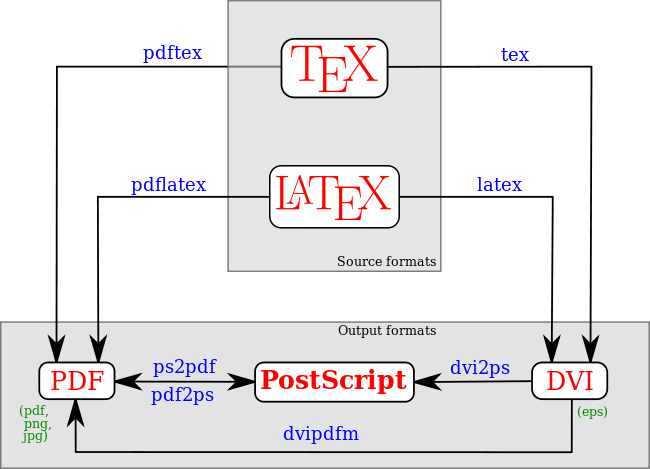
\includegraphics[scale=0.4]{img/650px-LaTeX_diagram}
\end{center}

\subsubsection{\LaTeX\ Distributions}
There are pre-compiled \LaTeX\ distributions for different OS:
\begin{itemize}
	\item TeX Live (Unix-like systems): Linux, BSD, Solaris, etc.
	\item MacTeX (TeX Live with the addition of Mac specific programs): \url{http://www.tug.org/mactex}
	\item MiKTeX (Windows): \url{http://www.miktex.org}
\end{itemize}

\subsection{Basic Structures}
\subsubsection{Document Structure}
The basic structure of \LaTeX\ file must contain the commands:

\begin{lstlisting}
	\documentclass{...}

	\begin{document}
		...
	\end{document}
\end{lstlisting}

The \emph{preamble} is the area between \\documentclass{...} and \\begin{document}, and contains commands and macros that affect the entire document.

The type of document is specified with \\documentclass mandatory command. 
\begin{lstlisting}
	\documentclass[options]{class}
\end{lstlisting}

There are the following document classes: article, report, book, slides, memoir, beamer, and letter (and special classes: IEEEtran, proc minimal).

And document class options are font size (10pt, 11pt, \dots), paper size, double o single side, and others.

There is another important optional command \\usepackage[option]{packages} to utilize external macros.

The \emph{document} environment includes document itself and information about itself (top matter), such as the title and date, and also information about the authors, such as name, address, email etc.

\begin{lstlisting}
	\begin{document}
		\title{How to Structure a LaTeX Document}
		\author{Andrew Roberts}	
		\date{December 2004}
		\maketitle
	\end{document}
\end{lstlisting}

As most research papers have an \emph{abstract}, there are predefined commands for telling LaTeX which part of the content makes up the abstract. 

\LaTeX\  provides 7 levels of depth for defining sections
\begin{center}
	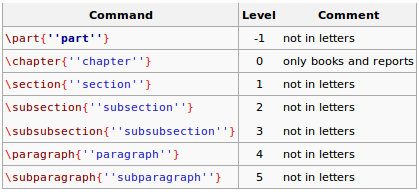
\includegraphics[scale=0.7]{img/levelSectionLatex}
\end{center}



\subsubsection{Fonts}
Fonts are a complex topic. For common documents, only Font families, Emphasizing text, and Font encoding are really needed. There are many font families e.g. Computer Modern, Times, Arial and Courier. Each family has its own font characteristics (such as italic and bold), also known as font styles, or font properties.

\begin{lstlisting}
	\textit { ... } % italics
	\textbf { ... } % bold
	\texttt { ... } % monospace - teletype
	\textsc { ... } % small capitals
\end{lstlisting}

Size related to font size default, declared in preamble (documentclass), and writer can use the following font sizes: tiny, scriptsize, footnotesize, small, normalsize, large, Large, LARGE, huge, and Huge.

\begin{center}
	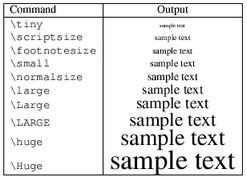
\includegraphics[scale=1]{img/sizingText}
\end{center}


For example,

\begin{lstlisting}
\LaTeX{} was \tiny originally written \normalsize 
in \large 1984 \normalsize by \LARGE Leslie Lamport 
\normalsize and has become the \footnotesize
dominant method \normalsize for using \huge \TeX. 
\end{lstlisting}

And the output

\LaTeX{} was \tiny originally written \normalsize in \large 1984 \normalsize by \LARGE Leslie Lamport \normalsize and has become the \footnotesize dominant method \normalsize for using \huge \TeX. 
\normalsize
\\
Some special features:
\begin{itemize}
    \item Text aligned.
    \item n$>$1 blank lines and empty spaces: one line or one space.
    \item Start a new paragraph: $\backslash\backslash$
    \item Hyphenate the word (exceptional cases): man$\backslash-u\backslash-$script.
    \item newline, newpage
\end{itemize}

\subsubsection{Environments}
In \LaTeX\ there is the possibility to mark block (text between begin and end commands) of text using different environment, such as centre, itemize, enumerate, figure, flushright, quotation, \dots.

For example, a enumerate list of items

\begin{lstlisting}
	Some FOSS License:
	\begin{enumerate}
		\item BSD license
		\item GPL license
		\item CDDL license
	\end{enumerate}
\end{lstlisting}
 
 And the output
 \\
 	Some FOSS License:
	\begin{enumerate}
		\item BSD license
		\item GPL license
		\item CDDL license
	\end{enumerate}
 

\subsection{Word Processors: Stupid and Inefficient}
In this article, Allin Cottrell writes about the differences between word processors and text editor, and claims that there are alternatives to editing text efficiently. She explains the importance of separating composition and typesetting, and advantages of using ASCII texts. He highlights that text is designed to communicated information, usually in two formats printing copies and digital copies. 

En general, a author does not really need that his text appears in nicely printed form when he is writing, usually after it is when he wants to print or send it.  Microsoft Word is the "natural" way to do all this, it's one way, but not the best.

Combine composition and typesetting task at the same time is not a effectively way to create and edit a text. Composition is the task of choice of words to express ideas, and the logical structuring of the text. On the other hand, typesetting is the task of choice  the font family, and the way in which structural elements will be visually represented. The author suggests that author should be two distinct "moments" in the production of a printed text using a computer.

Word processor forces you to complete two tasks in the same time the composition of the text itself and the typesetting of the document. An the author believes that it is not the most efficient way to create a document, because the author gets distracted with details and forgets the important aspects of text, such as composition and logical structuring of text. The author of a text should, at least in the first instance, concentrate entirely on the first of these sets of tasks. Besides, this procedure permits to he division of labour, and in this way professionalization of different tasks.

Current WYSIWYG ("What You See Is What You Get") word processor can make both tasks, but with some problems: The author is distracted from the proper business of composing text, WYSIWYG word processor sacrifices quality typesetting on screen to the speed, and losing sight of the logical structure of the text. What's more about the last problem, the logical structure is not explicit in the text (there are not metainformation), and when the author want to change the structure it is usually to make mistakes.

In relation to editor, word processor use binary formatting code and a text editor does not insert any binary formatting codes, representing features such as italics you have to do this via mark-up. Using text in plain ASCII using a text editor has the following advantages: Portability,  compactness, and security.

\LaTeX\ has the ability to change the typeset appearance of your text drastically and consistently with just a few commands. 
 
In relation to digital transmission, with simple documents the usage of plain text is an effective and economical way of communication (maybe nowadays with wide bandwidth this is different). On the other hand, in complex documents, such as mathematical text, there are some options: Convert the \TeX\ source file to HTML, convert to postscript file, or convert to pdf format.


\newpage
%------------------------------------------------------------------------------
% 2. MariaDB
\section{MariaDB}

\subsection{Introduction}
MariaDB is a community-developed "branch" or fork of the MySQL relational database management system, with the aim of being the community maintenance of its free status under the GNU GPL. MariaDB is a backward compatible and drop-in replacement for the MySQL Database server.

MariaDB strives to be the logical choice for database professionals looking for a robust, scalable, and reliable SQL server. To accomplish this, the MariaDB Foundation work closely and cooperatively with the larger community of users and developers in the true spirit of Free and open source software, and release software in a manner that balances predictability with reliability. 

Its lead developer is \emph{Michael "Monty" Widenius}, the founder of MySQL and Monty Program AB. He said that MariaDB is a branch of MySQL because now is 100\% compatible with MySQL.

The main features:
\begin{itemize}
	\item Open Source (First available from Launchpad, and nowadays from GitHub)
	\item Open bugs database (In contrast with MySQL).
	\item Multi-Platform support.
	\item SQL compatibility.
	\item Supports several storage engines: Aria, XtraDB, PBXT, FederatedX, Cassandra, CONNECT, SEQUENCE, Spider, and others.
	\item Speed improvements: Optimize enhancements, faster and safer replication, indexies for the memory, Debug code, and others.
	\item Test cases and coverage improvements.
	\item Thread Pooling - 200k+ connections.
	\item Removal of mutexes.
	\item Virtual columns.
	\item Improvement in show explain plan using another thread.
	\item Freedom - No Enterprise/Pay features.
\end{itemize}

The compatibility with MySQL is 100\% compatible. Client libraries, client-server protocols, SQL dialect, replication master-slave are all similar. Data files are supported as long as its similar between versions. Tools are similar. XtraDB enabled by default.

The several communication channels in the community: Mail lists, coding hosting, bug database, and IRC(\#maria).

\subsection{History}
The main historical event:
\begin{itemize}
	\item 1983 First version of what would become MySQL Developed by Michael Widenius and David Axmark
	\item 1995 MySQL AB company founded
	\item 1995 First internal release of MySQL
	\item 2000 MySQl goes free software (GPL)
	\item 2005 MySQL 5.0
	\item 2008 Sun Microsystems acquires MySQL AB (for \$1bn)
	\item 2008 MySQL 5.1
	\item 2009 Oracle acquires Sun Microsystems 
	\item 2010 MariaDB 5.1 released
	\item 2011/09 Oracle starts to sell commercial extensions
	\item 2012/09 MySQL 5.5.28
	\item 2012/12 Michael Widenius, David Axmark, and Allan Larsson announced the creation of a foundation that would oversee the development of MariaDB.
	\item 2013 MariaDB10.0 released (currently, 10.0.11)
\end{itemize}

Currently, there are around world 30 core MySQL developers in MariaDB development.

\subsection{Installing MariaDB}
MariaDB 5.5 is included in 14.04, to install it you can do

\begin{lstlisting}[label=intall,caption=Install Command]
janague@metricsGrimoireHost:~$sudo apt-get install mariadb-server
\end{lstlisting}

In general for other versions of Ubuntu, here are the commands to run to add MariaDB to your system:

\begin{lstlisting}[label=intall,caption=1. Install the repo manager]
janague@metricsGrimoireHost:~$ sudo apt-get install 
python-software-properties
Reading package lists... Done
Building dependency tree      
Reading state information... Done
The following extra packages will be installed:
  python-pycurl unattended-upgrades
Suggested packages:
  libcurl4-gnutls-dev python-pycurl-dbg bsd-mailx
The following NEW packages will be installed
  python-pycurl python-software-properties unattended-upgrades
0 upgraded, 3 newly installed, 0 to remove and 66 not upgraded.
Need to get 97.6 kB of archives.
After this operation, 657 kB of additional disk space will be used.

...

Setting up python-pycurl (7.19.0-4ubuntu3) ...
Setting up python-software-properties (0.82.7.6) ...
\end{lstlisting}

\begin{lstlisting}[label=intall,caption=2. Import the GnuPG signing key]
janague@metricsGrimoireHost:~$ sudo apt-key adv --recv-keys --keyserver 
hkp://keyserver.ubuntu.com:80 0xcbcb082a1bb943db
Executing: gpg --ignore-time-conflict --no-options --no-default-keyring 
--secret-keyring /tmp/tmp.EjYqLFa95L --trustdb-name /etc/apt/trustdb.gpg 
--keyring /etc/apt/trusted.gpg --primary-keyring /etc/apt/trusted.gpg 
--recv-keys --keyserver hkp://keyserver.ubuntu.com:80 0xcbcb082a1bb943db
gpg: requesting key 1BB943DB from hkp server keyserver.ubuntu.com
gpg: key 1BB943DB: public key "MariaDB Package Signing Key 
<package-signing-key@mariadb.org>" imported
gpg: no ultimately trusted keys found
gpg: Total number processed: 1
gpg:               imported: 1
janague@metricsGrimoireHost:~$ sudo add-apt-repository 
'deb http://ftp.igh.cnrs.fr/pub/mariadb/repo/5.5/ubuntu precise main'
\end{lstlisting}

\begin{lstlisting}[label=intall,caption=3. Refresh your system]
janague@metricsGrimoireHost:~$ sudo apt-get update
Hit http://es.archive.ubuntu.com precise Release.gpg
Hit http://es.archive.ubuntu.com precise-updates Release.gpg                  
Hit http://es.archive.ubuntu.com precise-backports Release.gpg                
Hit http://es.archive.ubuntu.com precise Release 

...

Hit http://es.archive.ubuntu.com precise-backports/multiverse 
Translation-en
Hit http://es.archive.ubuntu.com precise-backports/restricted 
Translation-en
Hit http://es.archive.ubuntu.com precise-backports/universe 
Translation-en
Fetched 11.5 kB in 1s (6,567 B/s)
Reading package lists... Done
\end{lstlisting}

\begin{lstlisting}[label=intall,caption=4. And finally install MariaDB]
janague@metricsGrimoireHost:~$ sudo apt-get install mariadb-server
Reading package lists... Done
Building dependency tree      
Reading state information... Done
The following extra packages will be installed:
  libaio1 libdbd-mysql-per\begin{itemize}l libdbi-perl libhtml-template-perl
...
 * Starting MariaDB database server mysqld                               [ OK ]
 * Checking for corrupt, not cleanly closed and upgrade needing tables.
Setting up mariadb-server (5.5.34+maria-1~precise) ...
Processing triggers for libc-bin ...
ldconfig deferred processing now taking place
\end{lstlisting}


\subsection{MariaDB command line client}
MariaDB command line client is the command \emph{mysql} (the same spelling of MySQL). it is a simple SQL shell, which supports interactive and noninteractive use. 

Invoking it from the prompt of your command interpreter as follows:

\begin{lstlisting}[label=intall,caption=mysql interpreter]
janague@metricsGrimoireHost:~$ mysql -u root -p
Enter password: 
Welcome to the MariaDB monitor.  Commands end with ; or \g.
Your MariaDB connection id is 93
Server version: 5.5.34-MariaDB-1~precise-log mariadb.org binary 
distribution

Copyright (c) 2000, 2013, Oracle, Monty Program Ab and others.

Type 'help;' or '\h' for help. Type '\c' to clear the current 
input statement.

MariaDB [(none)]> 
\end{lstlisting}

\begin{lstlisting}[label=option,caption=mysql option]
Command:
	mysql [<options>] database
Common options:
	--user, -u: MySQL user name
	--password, -p: user's password
	--host, -h: connect to the server on the given host
\end{lstlisting}

The full list of supported options can be obtained with:
\begin{lstlisting}
janague@metricsGrimoireHost:~$ mysql --verbose --help
mysql  Ver 15.1 Distrib 5.5.34-MariaDB, for debian-linux-gnu (x86_64) 
using readline 5.1
Copyright (c) 2000, 2013, Oracle, Monty Program Ab and others.

Usage: mysql [OPTIONS] [database]
  -?, --help          Display this help and exit.
  -I, --help          Synonym for -?
  --abort-source-on-error 
                      Abort 'source filename' operations in case 
                      of errors
...
max-join-size                     1000000
secure-auth                       FALSE
show-warnings                     FALSE
plugin-dir                        (No default value)
default-auth                      (No default value)
binary-mode                       FALSE
\end{lstlisting}

And also using man command.

\subsection{MariaDB commands}
Here we show the basic commands
\begin{lstlisting}[label=basic_command,caption=Show and create a Database]
janague@metricsGrimoireHost:~$ mysql -u root -p

Enter password:
Welcome to the MariaDB monitor.  Commands end with ; or \g.

Your MariaDB connection id is 30

Server version: 5.5.34-MariaDB-1~precise-log mariadb.org binary 
distribution

Copyright (c) 2000, 2013, Oracle, Monty Program Ab and others.
Type 'help;' or '\h' for help. Type '\c' to clear the current input 
statement.
MariaDB [(none)]> create user 'janague'@'localhost' identified by
 'janague123';
Query OK, 0 rows affected (0.00 sec)

MariaDB [(none)]> show databases;
+--------------------+
| Database           |
+--------------------+
| information_schema |
| mysql              |
| performance_schema |
+--------------------+
3 rows in set (0.00 sec)

MariaDB [(none)]> create database csiDB;
Query OK, 1 row affected (0.00 sec)

MariaDB [(none)]> show databases;
+--------------------+
| Database     \begin{itemize}      |
+--------------------+
| information_schema |
| csiDB              |
| mysql              |
| performance_schema |
+--------------------+
4 rows in set (0.00 sec)
\end{lstlisting}

\begin{lstlisting}[label=basic_command,caption=Drop a Database]
MariaDB [(none)]> drop database csiDB;
Query OK, 0 rows affected (0.01 sec)

ariaDB [(none)]> show databases;
+--------------------+
| Database           |
+--------------------+
| information_schema |
| mysql              |
| performance_schema |
+--------------------+
3 rows in set (0.00 sec)
\end{lstlisting}

\begin{lstlisting}[label=basic_command,caption=Change of Database]
MariaDB [(none)]> create database csiDB;
Query OK, 1 row affected (0.00 sec)

MariaDB [(none)]> use csiDB;
Database changed
MariaDB [csiDB]> show tables;
Empty set (0.00 sec)
\end{lstlisting}

\begin{lstlisting}[label=basic_command,caption=Create and show a table ]
MariaDB [csiDB]> CREATE TABLE IF NOT EXISTS equipment (
    ->     equip_id int(5) NOT NULL AUTO_INCREMENT,
    ->     type varchar(50) DEFAULT NULL,
    ->     install_date DATE DEFAULT NULL,
    ->     PRIMARY KEY(equip_id)
    ->     );
Query OK, 0 rows affected (0.01 sec)

MariaDB [csiDB]> show tables;
+-----------------+
| Tables_in_csiDB |
+-----------------+
| equipment       |
+-----------------+
1 row in set (0.00 sec)
    
\end{lstlisting}

\begin{lstlisting}[label=basic_command,caption=Table description]
MariaDB [csiDB]> desc equipment;
+--------------+-------------+------+-----+---------+----------------+
| Field        | Type        | Null | Key | Default | Extra          |
+--------------+-------------+------+-----+---------+----------------+
| equip_id     | int(5)      | NO   | PRI | NULL    | auto_increment |
| type         | varchar(50) | YES  |     | NULL    |                |
| install_date | date        | YES  |     | NULL    |                |
+--------------+-------------+------+-----+---------+----------------+
3 rows in set (0.01 sec)

MariaDB [csiDB]> show fields from equipment;
+--------------+-------------+------+-----+---------+----------------+
| Field        | Type        | Null | Key | Default | Extra          |
+--------------+-------------+------+-----+---------+----------------+
| equip_id     | int(5)      | NO   | PRI | NULL    | auto_increment |
| type         | varchar(50) | YES  |     | NULL    |                |
| install_date | date        | YES  |     | NULL    |                |
+--------------+-------------+------+-----+---------+----------------+
3 rows in set (0.00 sec)

    
\end{lstlisting}


\subsection{Administration}
\emph{mysqladmin} is an administration program for the mysqld daemon. It can be used to:
\begin{itemize}
    \item Monitor what the MySQL clients are doing (processlist)
    \item Get usage statistics and variables from the MariaDB / MySQL server
    \item Create/drop databases
    \item Flush (reset) logs, statistics and tables
    \item Kill running queries.
    \item Stop the server (shutdown)
    \item Start/stop slaves
    \item Check if the server is alive (ping) 
\end{itemize}

\begin{lstlisting}[label=basic_command,caption=Create Database]
janague@metricsGrimoireHost:~$ mysqladmin -u root -p create csiDB2
Enter password: 
janague@metricsGrimoireHost:~$ mysql -u root -p
password:
...
MariaDB [(none)]> show databases;
+--------------------+
| Database           |
+--------------------+
| information_schema |
| csiDB              |
| csiDB2             |
| mysql              |
| performance_schema |
+--------------------+
5 rows in set (0.00 sec)

MariaDB [csiDB]> exit
Bye
\end{lstlisting}

\begin{lstlisting}[label=basic_command,caption=Drop Database]
janague@metricsGrimoireHost:~$ mysqladmin -u root -p drop csiDB2
Enter password: 
Dropping the database is potentially a very bad thing to do.
Any data stored in the database will be destroyed.

Do you really want to drop the 'csiDB2' database [y/N] y
Database "csiDB2" dropped
janague@metricsGrimoireHost:~$ 

janague@metricsGrimoireHost:~$ mysql -u root -p
password:
...
MariaDB [(none)]> show databases;
+--------------------+
| Database           |
+--------------------+
| information_schema |
| csiDB              |
| mysql              |
| performance_schema |
+--------------------+
4 rows in set (0.00 sec)

MariaDB [csiDB]> exit
Bye
\end{lstlisting}

\begin{lstlisting}[label=basic_command,caption=Show Variables]
janague@metricsGrimoireHost:~$ mysqladmin -u root -p variables
| Variable_name                                     | Value 
| aria_block_size                                   | 8192    
| aria_checkpoint_interval                          | 30 
...
| version_compile_os                                | debian-linux-gnu 
| wait_timeout                                      | 600     
\end{lstlisting}


\subsection{Backup}
The \emph{mysqldump} client can be used to dump a database or a collection of databases for backup or transfer to another database server (not necessarily MariaDB or MySQL). The dump typically contains SQL statements to create the table, populate it, or both. However, mysqldump can also be used to generate files in CSV, other delimited text, or XML format.

\begin{lstlisting}[label=basic_command,caption=Backup Database]
janague@metricsGrimoireHost:~$ mysqldump -u root -p csiDB equipment
Enter password: 
-- MySQL dump 10.14  Distrib 5.5.34-MariaDB, for debian-linux-gnu 
(x86_64)
--
-- Host: localhost    Database: csiDB
-- ------------------------------------------------------
-- Server version	5.5.34-MariaDB-1~precise-log

/*!40101 SET @OLD_CHARACTER_SET_CLIENT=@@CHARACTER_SET_CLIENT */;
/*!40101 SET @OLD_CHARACTER_SET_RESULTS=@@CHARACTER_SET_RESULTS */;
...

--
-- Table structure for table `equipment`
--

DROP TABLE IF EXISTS `equipment`;
/*!40101 SET @saved_cs_client     = @@character_set_client */;
/*!40101 SET character_set_client = utf8 */;
CREATE TABLE `equipment` (
  `equip_id` int(5) NOT NULL AUTO_INCREMENT,
  `type` varchar(50) DEFAULT NULL,
  `install_date` date DEFAULT NULL,
  PRIMARY KEY (`equip_id`)
) ENGINE=InnoDB DEFAULT CHARSET=latin1;
/*!40101 SET character_set_client = @saved_cs_client */;

...
  /*!40101 SET SQL_MODE=@OLD_SQL_MODE */;
/*!40014 SET FOREIGN_KEY_CHECKS=@OLD_FOREIGN_KEY_CHECKS */;
/*!40014 SET UNIQUE_CHECKS=@OLD_UNIQUE_CHECKS */;
/*!40101 SET CHARACTER_SET_CLIENT=@OLD_CHARACTER_SET_CLIENT */;
/*!40101 SET CHARACTER_SET_RESULTS=@OLD_CHARACTER_SET_RESULTS */;
/*!40101 SET COLLATION_CONNECTION=@OLD_COLLATION_CONNECTION */;
/*!40111 SET SQL_NOTES=@OLD_SQL_NOTES */;

-- Dump completed on 2014-05-05  3:34:56
  
\end{lstlisting}

\begin{lstlisting}[label=basic_command,caption=Restore Database]
janague@metricsGrimoireHost:~$ mysqladmin -u root -p drop csiDB
Enter password: 
Dropping the database is potentially a very bad thing to do.
Any data stored in the database will be destroyed.

Do you really want to drop the 'csiDB' database [y/N] y
Database "csiDB" dropped

janague@metricsGrimoireHost:~$ mysqladmin -u root -p create csiDB
Enter password: 

janague@metricsGrimoireHost:~$ mysql -u root -p csiDB < backup_file.sql 
Enter password: 

janague@metricsGrimoireHost:~$ mysql -u root -p
password:
...
MariaDB [(none)]> show databases;
+--------------------+
| Database           |
+--------------------+
| information_schema |
| csiDB              |
| mysql              |
| performance_schema |
+--------------------+
4 rows in set (0.00 sec)

MariaDB [(none)]> use csiDB;
Reading table information for completion of table and column names
You can turn off this feature to get a quicker startup with -A

Database changed
MariaDB [csiDB]> show tables;
+-----------------+
| Tables_in_csiDB |
+-----------------+
| equipment       |
+-----------------+
1 row in set (0.00 sec)

MariaDB [csiDB]> exit
Bye
\end{lstlisting}

There are other options to back up multiples databases (mysqldump [<options>] \textbf{--databases} [<db> <db> ...]), back up all databases in the server (mysqldump [<options>] \textbf{--all-databases} [<options>], and )

\subsection{GUI tools}
 There are many GUI tools that work with MariaDB, such as Webyog/SQLyog, HeidiSQL, and of course, MySQL Workbench.
 
 \emph{phpMyAdmin} is a free software tool written in PHP, intended to handle the administration of MySQL over the Web. phpMyAdmin supports a wide range of operations on MySQL, \emph{MariaDB} and Drizzle.
 
 \begin{lstlisting}[label=gui_tools,caption=Install phpMyAdmin]
janague@metricsGrimoireHost:~$ sudo apt-get install phpmyadmin
Reading package lists... Done
Building dependency tree       
Reading state information... Done
The following extra packages will be installed:
  apache2-mpm-prefork apache2-utils apache2.2-bin apache2.2-common dbconfig-common libapache2-mod-php5 libapr1
  libaprutil1 libaprutil1-dbd-sqlite3 libaprutil1-ldap libcap2 libgd2-xpm libmcrypt4 libt1-5 php5-cli php5-common
  php5-gd php5-mcrypt php5-mysql ssl-cert

...

dbconfig-common: flushing administrative password
 * Reloading web server config apache2                                                                                  apache2: Could not reliably determine the server's fully qualified domain name, using 127.0.1.1 for ServerName
                                                                                                                 [ OK ]
Processing triggers for libc-bin ...
ldconfig deferred processing now taking place

 \end{lstlisting}
 
\begin{center}
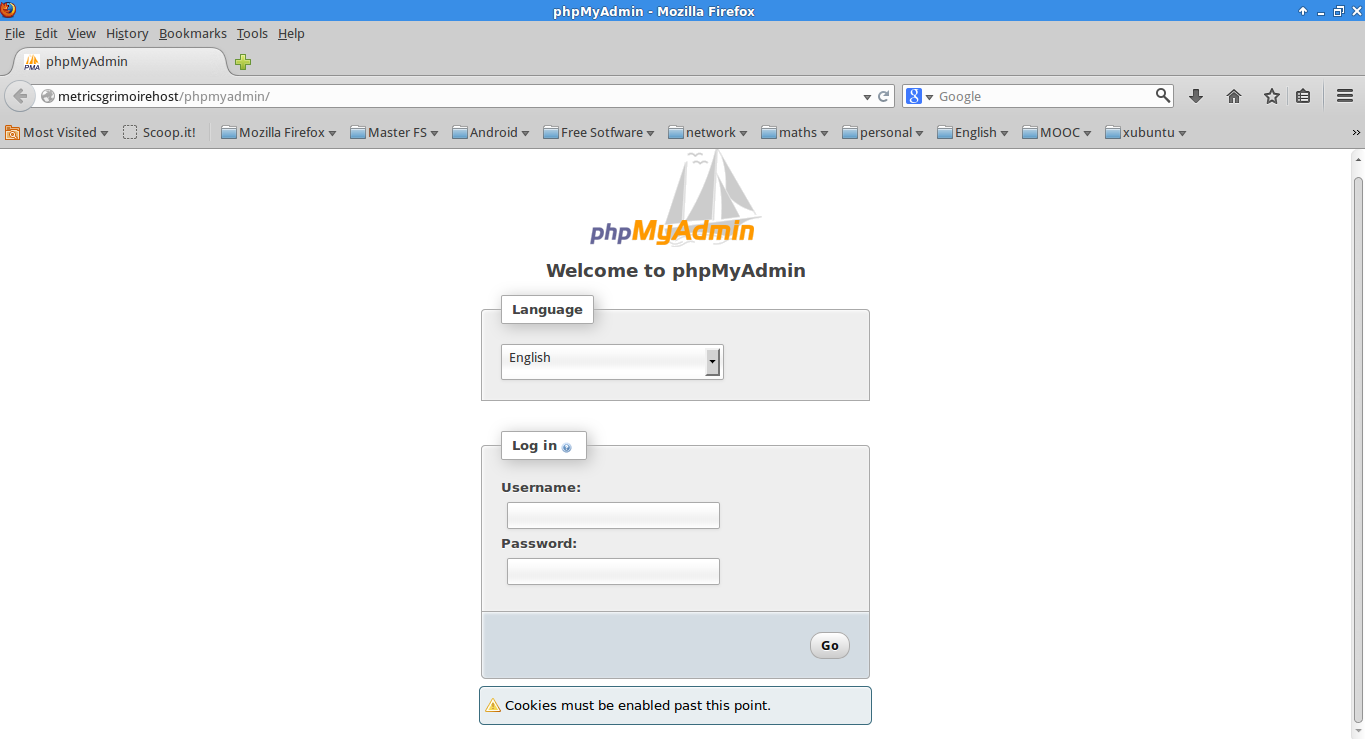
\includegraphics[scale=0.3]{img/phpmyadmin}
\end{center}
\begin{center}
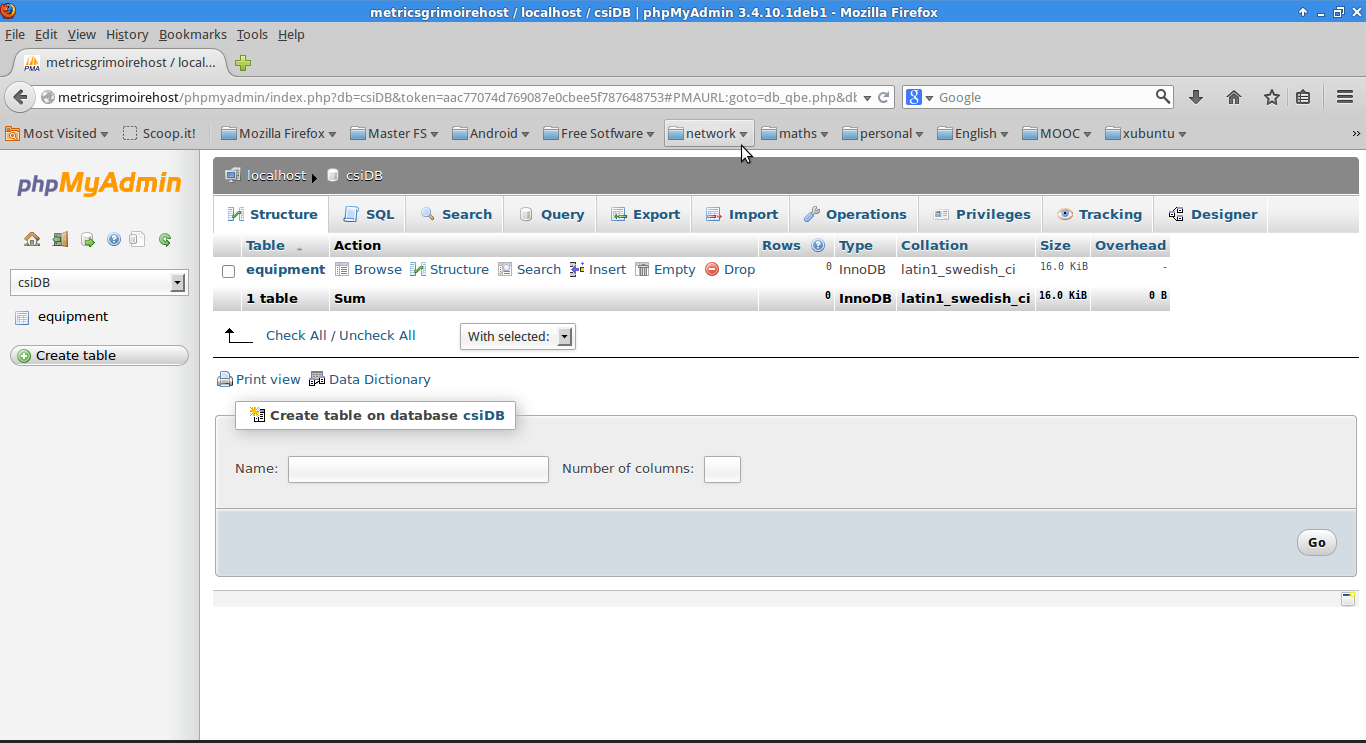
\includegraphics[scale=0.3]{img/phpmyadmin_csi}
\end{center}
 
\newpage

 %------------------------------------------------------------------------------
% 3. GNU R
\section{GNU R}

\subsection{Introduction}
R is \emph{a language and environment for statistical computing and graphics}. R is an integrated suite of software facilities for data manipulation, calculation and graphical
display. It is a GNU project (GNU GPL v2) which is similar to the S language and environment which was developed at Bell Laboratories (formerly AT\&T, now Lucent Technologies) by John Chambers, Robert Gentleman, Ross Ihaka, and others. It is a powerful language and easy to use. 

R is available as Free Software under the terms of the Free Software Foundation's GNU General Public License in source code form. It compiles and runs on \emph{multiple operating systems}, such as UNIX platforms and similar systems (including FreeBSD and Linux), Windows and MacOS. 

R provides \emph{a wide variety of statistical} (linear and nonlinear modelling, classical statistical tests, time-series analysis, classification, clustering, ...) and graphical techniques, and is highly extensible. The S language is often the vehicle of choice for research in statistical methodology. 

R can be \emph{extended easily via packages}. There are about eight packages supplied with the R distribution and many more are available through the \emph{CRAN} (The Comprehensive R Archive Network) family of Internet sites covering a very wide range of modern statistics.

The current R is the result of a collaborative effort with contributions from all over the world. R was initially written by Robert Gentleman and Ross Ihaka—also known as "R \& R" of the Statistics Department of the University of Auckland. R provides an Open Source route to participation in that activity. There is a core group with write access to the R source code, currently consisting of 22 members. Besides, there are many others that contributed by donating code, bug fixes and documentation.
   
    The R Foundation is a not for profit organization that holds and administers the copyright of R software and documentation. The principal organs of the “R Foundation” are: The general assembly, the board, the auditors, and the court of arbitration.
 
\subsection{Installation} 
To obtain the latest R packages, add an entry like

 \begin{lstlisting}
   deb http://<my.favorite.cran.mirror>/bin/linux/ubuntu saucy/
 \end{lstlisting}
 
 In /etc/apt/sources.list file, replacing
<my.favorite.cran.mirror> by the actual URL of your favorite CRAN
mirror. See http://cran.r-project.org/mirrors.html for the list of
CRAN mirrors. To install the complete R system, use

 \begin{lstlisting}
   sudo apt-get update
   sudo apt-get install r-base
 \end{lstlisting}
 
 
\subsection{Getting Help} 
First, to start the R program with the command
 \begin{lstlisting}
   $ R
 \end{lstlisting}
 
To quit the R program the command is

\begin{lstlisting}
   > q()
\end{lstlisting}

\begin{lstlisting}[caption=Start R and Quit]
janague@gon:~/Documents/mswl/mswl_csi/R/work$ R

R version 3.0.1 (2013-05-16) -- "Good Sport"
Copyright (C) 2013 The R Foundation for Statistical Computing
Platform: x86_64-pc-linux-gnu (64-bit)

R is free software and comes with ABSOLUTELY NO WARRANTY.
You are welcome to redistribute it under certain conditions.
Type 'license()' or 'licence()' for distribution details.

  Natural language support but running in an English locale

R is a collaborative project with many contributors.
Type 'contributors()' for more information and
'citation()' on how to cite R or R packages in publications.

Type 'demo()' for some demos, 'help()' for on-line help, or
'help.start()' for an HTML browser interface to help.
Type 'q()' to quit R.

> q()
Save workspace image? [y/n/c]: y
janague@gon:~/Documents/mswl/mswl_csi/R/work$ 
\end{lstlisting}
 
R has an inbuilt help facility to get information on any specific function.
  \begin{lstlisting}
   > help(funcName)
 \end{lstlisting}
 an alternative is 
  \begin{lstlisting}
   > ?funcName
 \end{lstlisting}
 
On most R installations help is available in HTML format by running
  \begin{lstlisting}
> help.start()
 \end{lstlisting}
 
\begin{center}
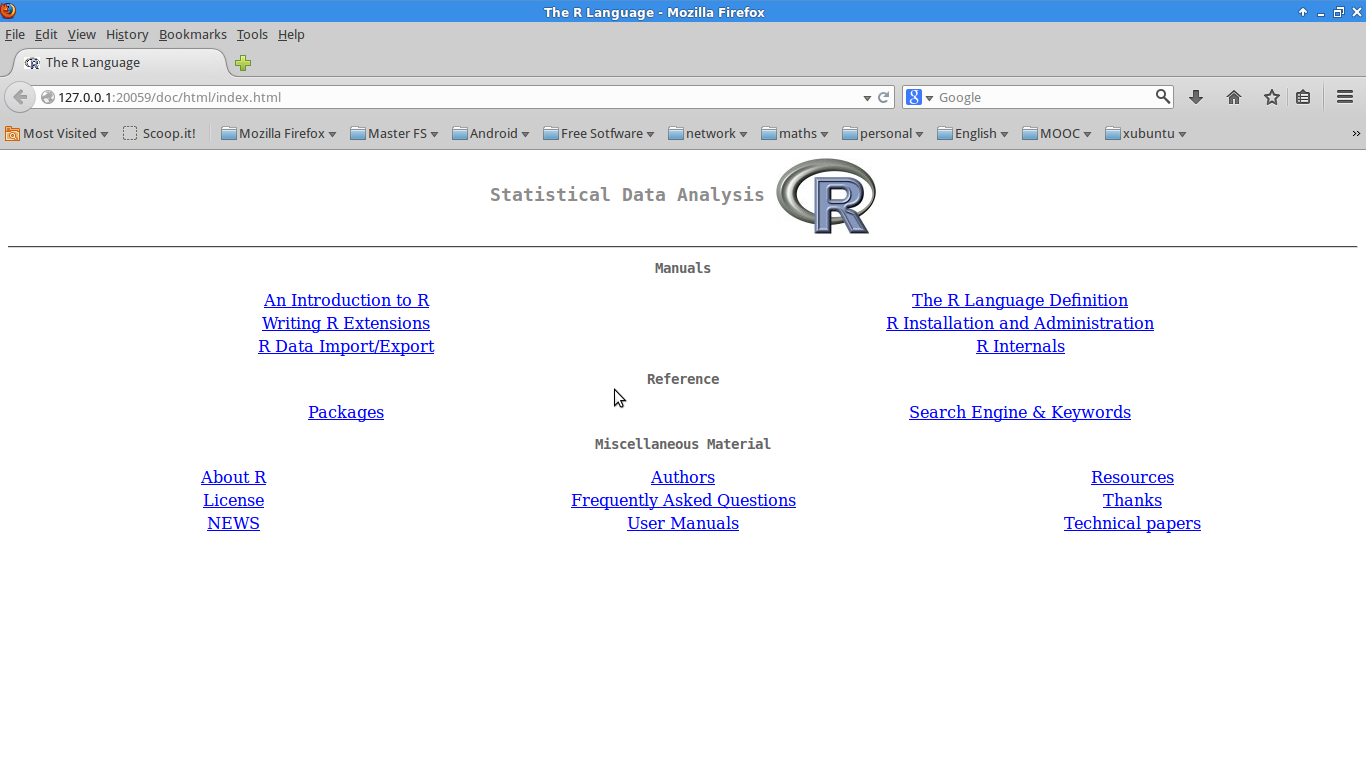
\includegraphics[scale=0.3]{img/Rstart}
\end{center}
 
The help.search command (alternatively ??) allows searching for help in various ways. For example,
  \begin{lstlisting}[caption=Help Search]
> help.search("solve")

Help files with alias or concept or title matching 'solve' using 
fuzzy matching:

base::backsolve         Solve an Upper or Lower Triangular System
base::qr                The QR Decomposition of a Matrix
base::solve             Solve a System of Equations
...
 \end{lstlisting}
 
 Finally, to get information about library we can use library command
   \begin{lstlisting}[caption=Library command]
> library(help=MASS)
                Information on package 'MASS'

Description:

Package:            MASS
Priority:           recommended
Version:            7.3-27
Date:               2013-07-01
Revision:           $Rev: 3322 $
Depends:            R (>= 3.0.0), grDevices, graphics, stats, utils
Suggests:           lattice, nlme, nnet, survival
Authors@R:          c(person("Brian", "Ripley", role = c("aut", 

...
 \end{lstlisting}
 
\subsection{R libraries} 
Packages stores all R functions and datasets, only when a package is loaded are its
contents available.

To see which packages are installed at your site, library command is used with no arguments.
\begin{lstlisting}[caption=Installed Packages]
> library()

Packages in library '/home/janague/R/x86_64-pc-linux-gnu-library/3.0':

DBI                     R Database Interface
manipulate              Interactive Plots for RStudio
rstudio                 Tools and Utilities for RStudio

Packages in library '/usr/lib/R/site-library':

DBI                     R Database Interface

Packages in library '/usr/lib/R/library':

base                    The R Base Package
boot                    Bootstrap Functions (originally by Angelo Canty
                        for S)
class                   Functions for Classification
...

\end{lstlisting}

To install and update packages we can use the install.packages() and update.packages() commands. And command search() to see which packages are currently loaded.

\begin{lstlisting}[caption=Search command]
> search()
 [1] ".GlobalEnv"        "package:MASS"      "package:stats"    
 [4] "package:graphics"  "package:grDevices" "package:utils"    
 [7] "package:datasets"  "package:methods"   "Autoloads"        
[10] "package:base"  
\end{lstlisting}

The standard (or base) packages are considered part of the R source code. Besides, there are thousands of contributed packages for R, written by many different authors, most are available for download from CRAN (\url{http://CRAN.R-project.org/})

\subsection{R scripts} 
R commands can store in an external file with extension ".r" or ".R" and execute with the command source, in that way we can create scripts.

  \begin{lstlisting}
> source("commands.R")
 \end{lstlisting}

Also, it is possible to execute from the command-line 

\begin{lstlisting}[caption=R Scripts]
janague@gon:~/Documents/mswl/mswl_csi/R/work$ more commands.R 
a=1; b=2; c=3; a+b/c
janague@gon:~/Documents/mswl/mswl_csi/R/work$ R --vanilla < commands.R

R version 3.0.1 (2013-05-16) -- "Good Sport"
Copyright (C) 2013 The R Foundation for Statistical Computing
Platform: x86_64-pc-linux-gnu (64-bit)

R is free software and comes with ABSOLUTELY NO WARRANTY.
You are welcome to redistribute it under certain conditions.
Type 'license()' or 'licence()' for distribution details.

  Natural language support but running in an English locale

R is a collaborative project with many contributors.
Type 'contributors()' for more information and
'citation()' on how to cite R or R packages in publications.

Type 'demo()' for some demos, 'help()' for on-line help, or
'help.start()' for an HTML browser interface to help.
Type 'q()' to quit R.

> a=1; b=2; c=3; a+b/c
[1] 1.666667
> 
janague@gon:~/Documents/mswl/mswl_csi/R/work$ 
\end{lstlisting}

\subsection{Operations and Vectors} 
R operates on named data structures . The simplest such structure is the numeric vector, which is a single entity consisting of an ordered collection of numbers.

\begin{lstlisting}[caption=Vectors]
> v1 = c(1,2,3,4,5)
> v1
[1] 1 2 3 4 5
> seq(1,20,2)
 [1]  1  3  5  7  9 11 13 15 17 19
\end{lstlisting}

Vectors can be used in arithmetic expressions, in which case the operations are performed element by element. And "$<-$" is an assignment statement.

\begin{lstlisting}[caption=Vectors Operations]
> v1
[1] 1 2 3 4 5
> v1 <- 2*v1 + 1
> v1
[1]  3  5  7  9 11
\end{lstlisting}

\subsection{Simple functions}
The elementary arithmetic operators are the usual +, -, *, / and \^\   for raising to a power. In addition all of the common arithmetic functions are available. \emph{log, exp, sin, cos, tan, sqrt}, and so on, all have their usual meaning. \emph{max} and \emph{min} select the largest and smallest elements of a vector respectively. range is a function whose value is a vector of length two, namely \emph{c(min(x), max(x))}. \emph{length(x)} is the number of elements in x, sum(x) gives the total of the elements in x, and prod(x) their product. Two statistical functions are \emph{mean(x)} which calculates the sample mean.

\begin{lstlisting}[caption=Simple Functions]
> length(v1)
[1] 5
> mean(v1)
[1] 7
> sum(v1)
[1] 35
> median(v1)
[1] 7
> summary(v1)
   Min. 1st Qu.  Median    Mean 3rd Qu.    Max. 
      3       5       7       7       9      11 

\end{lstlisting}

\subsection{Graphs in R}
Graphical facilities are an important and extremely versatile component of the R environment. It is possible to use the facilities to display a wide variety of statistical graphs and also to build entirely new types of graph. 

One of the most frequently used plotting functions in R is the plot() function. This is a generic function: the type of plot produced is dependent on the type or class of the first argument. 

\begin{lstlisting}[caption=Plot Function]
> library(MASS)
> plot(Animals$body, Animals$brain, log="xy")
\end{lstlisting}
with the following output
\begin{center}
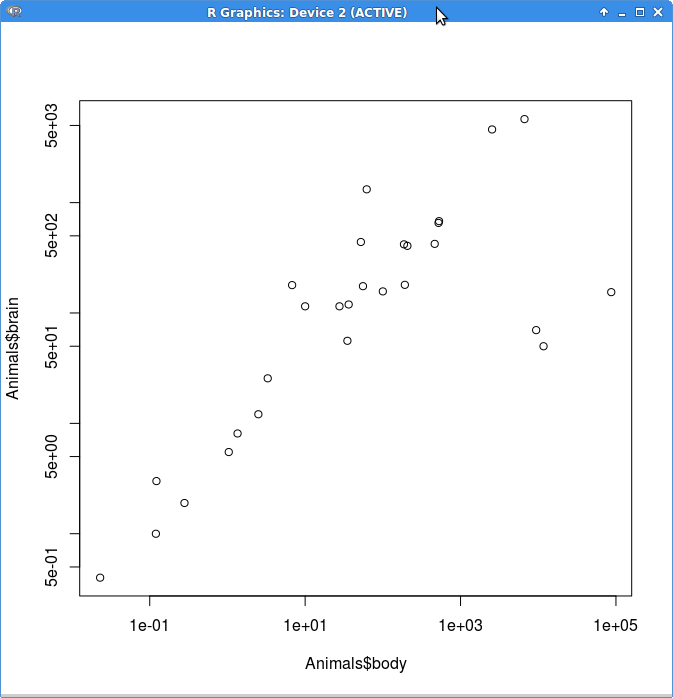
\includegraphics[scale=0.4]{img/plotFunction}
\end{center}

Others functions called low-level plotting commands can be used to add extra information (such as points, lines or text) to the current plot.
\begin{lstlisting}[caption=Low-level Plotting Commands]
> with(Animals, plot(body, brain, log="xy", col="navy", xlab="body",
 ylab="brain", main="brain vs. body"))
> text(1e+03,5, paste("By the way, v1[1] = ", v1[1]))
> abline(lm(log10(Animals$brain)~log10(Animals$body)), col="red")
\end{lstlisting}

\begin{center}
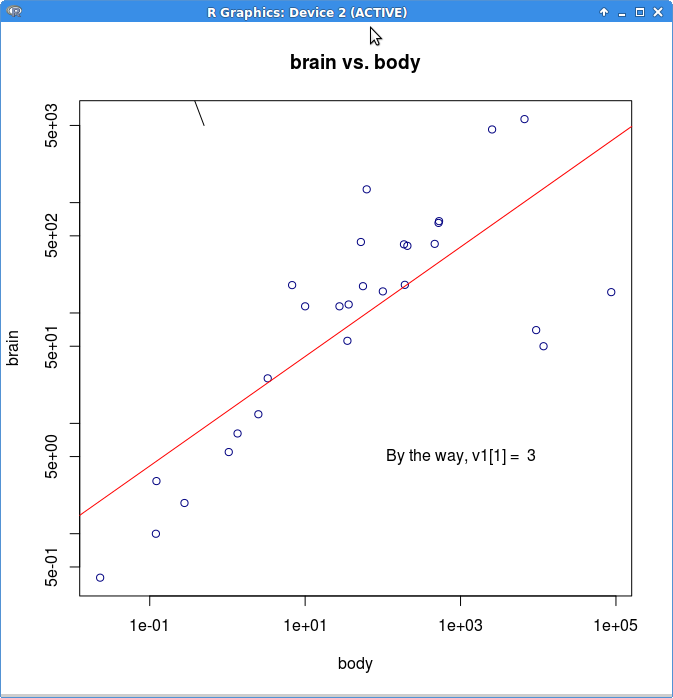
\includegraphics[scale=0.4]{img/LowLevelPlotFunction}
\end{center}

Another example with histogram function
\begin{lstlisting}[caption=Histogram and Kernel Density Estiamtion]
> hist(rnorm(n=5000, m=2, sd=2), freq=F, main = "Histogram and KDE 
of Gaussiand dist.")
> lines(density((rnorm(n=5000, m=2, sd=2)), col="red", lwd=2, lty=2))
\end{lstlisting}

\begin{center}
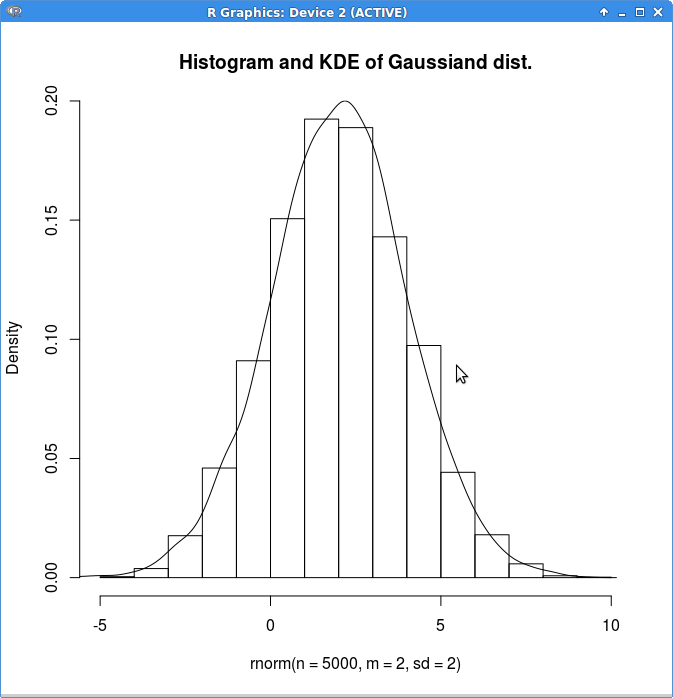
\includegraphics[scale=0.4]{img/histogram}
\end{center}

\newpage

%------------------------------------------------------------------------------
% 4. Translation in Libre Software
\section{Translation in Libre Software}

\subsection{Introduction}
Software \emph{internationalization} is the process to prepare a program to be adapted to different languages, regional or cultural differences without engineering changes (source code remains the same). 

\emph{Localization} refers to the adaptation of a product, application or document content to meet the language, cultural and other requirements of a specific target market (a locale). 

\emph{Translation} is to adapt the text to different languages, often thought of only as a synonym for translation of the user interface and documentation, localization is often a substantially more complex issue. Translation is only a part of the localization process.

\emph{Globalization} is the process to design and development methods for a product in advance, keeping in mind a multicultural audience, in order to avoid increased costs and quality problems, save time, and smooth the localizing effort for each region or country. And internationalization and localization are two primary technical processes that comprise globalization.

\begin{center}
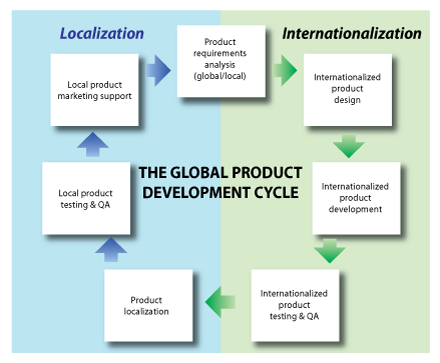
\includegraphics[scale=0.6]{img/globalCycle}
\end{center}

In free software project it is a perfect scenario for its freedom where anyone can translate part of the code and usually documentation too. 

\subsection{Localization}
Localization refers to the adaptation of a product, application or document content to meet the language, cultural and other requirements of a specific target market (a locale). Localization is sometimes referred to by the numeronym l10n (as in: “l”,  where 10 is the number of letters between l and n y word localization). 

Localization entails customization related to:
\begin{itemize}
    \item Numeric, date and time formats
    \item Use of currency
    \item Keyboard usage
    \item Collation and sorting
    \item Symbols, icons and colors
    \item Text and graphics containing references to objects, actions or ideas which, in a given culture, may be subject to misinterpretation or viewed as insensitive.
    \item Varying legal requirements
    \item others
\end{itemize}

Document localization life-cycle includes 
\begin{itemize}
	\item Prepare: Identify and define the objects to be localized
	\item Internationalize: Separate texts from source code, set up the accepted type of documents for translation
	\item Localize: Match the objects to be translated with previous translated versions of the project if possible. Translation of the pending strings QA/Post-editing of the translated objects.
	\item Publish: Update the original project integrating the target language
	\item Review, maintenance, and quality assurance
\end{itemize}

The main objects affected by localization may be messages in the code, help, documentation, installer, web side, wiki, and others.

In localization there are different techniques to achieve its tasks:
\begin{itemize}
	\item Standalone translation tools: Poedit (Gettext Translations Editor), Gtranslation, Lokalize (computer-aided translation system that focuses on productivity and quality assurance in KDE), Virtaal (computer-assisted translation tool written in the Python programming language. It is free software developed and maintained by Translate.org.za)
	\item Translation web platforms: Pootle (an online translation management tool with translation interface. It is written in the Python programming language using the Django framework and is free software originally developed and released by Translate.org.za), Launchpad, Transifex (a version-control system and repository for your global content, such as strings, video subtitles, landing pages and marketing emails), Weblate (a free web-based translation tool with tight Git integration)
	\item Other approaches: Editor add-ons, projects with built-in I10n tools: Drupal, Wordpress plugins
\end{itemize}

\subsection{Internationalization}
Internationalization is the process of designing a software application so that it can potentially be adapted to various languages and regions without engineering changes. . Internationalization is sometimes referred to by the numeronym i18n (as in: “i”, where 18 is the number of letters between i and n y word internationalization).
The internationalization process involve to developers and translators, and internalization team in large projects, where formats and coding guidelines should be accept for all. 

There are conventions in the file formats of internalization:
\begin{itemize}
	\item Plain text files
	\item \emph{gettext} is an internationalization and localization (i18n) system commonly used for writing multilingual programs on Unix-like computer operating systems. The most commonly used implementation of gettext is GNU gettext, released by the GNU Project in 1995.
	\begin{lstlisting}
printf(gettext("My name is %s.\n"), my_name);
	\end{lstlisting}
	In es.po file
	\begin{lstlisting}
msgid "My name is %s.\n"
msgstr "Mi nombre es %s.\n"
	\end{lstlisting}
	\item XLIFF (XML Localisation Interchange File Format) is an XML-based format created to standardize the way localizable data are passed between tools during a localization process.
\end{itemize}

\newpage


%------------------------------------------------------------------------------
% 5. Introduction to Unix shell
\section{Introduction to Unix shell}

\subsection{Introduction}
A Unix shell is a command-line \emph{interpreter} that provides a traditional user interface for the Unix operating system and for Unix-like systems. Users direct the operation of the computer by entering commands as text for a command line interpreter to execute, or by creating text scripts of one or more such commands. 

The stages of booting of a system and in particular in GNU/Linux are the following:

\begin{enumerate}
	\item \emph{System startup}: It is the first stage of booting process, the power is supplied to all the devices connected to that machine (motherboard, processor, hdd, cd-rom, mouse, etc). The processor starts running a sequence operations stored in its memory (ROM). The first instruction is to pass control to BIOS (Basic Input/Output System) to do POST (Power On Self Test), if all checks are ok,  the first boot device is selected from the stored list, and BIOS gives back the control to processor.
	\item \emph{Boot loader - MBR loading}: Before BIOS gives back control to processor, it tries to load MBR (Master Boot Recorder), which is a small part of HDD with just a size of 512 bytes. Primary boot loader code, the first 446 bytes of MBR, provides information and location details of actual boot loader on the hard disk to be loaded by CPU. MBR also contains 64 bytes of data which stores partition table information.
	\item \emph{Boot loader - GRUB loader}: GRUB is located in the first 30 kilobytes of hard disk immediately following the MBR is loaded into RAM for reading its configuration and displays OS boot menu.
	\item \emph{Kernel loading}: When user selects OS, kernel is loaded into to RAM and always resides on RAM until the machine is shutdown. The first operation that kernel executes is INIT process.
	\item \emph{INIT process}: INIT is the root/parent process of all the processes which run under GNU/Linux. It runs the following processes: /etc/rc.d/ rc.sysinit, based on the appropriate run-level it executes to start/stop various processes, read /etc/inittab, and /etc/rc.local the last process.
	\item \emph{User prompt}: Although it is actually no part of booting process it is important since it starts multiple of instances of getty waiting for console logins.
\end{enumerate}

\begin{center}
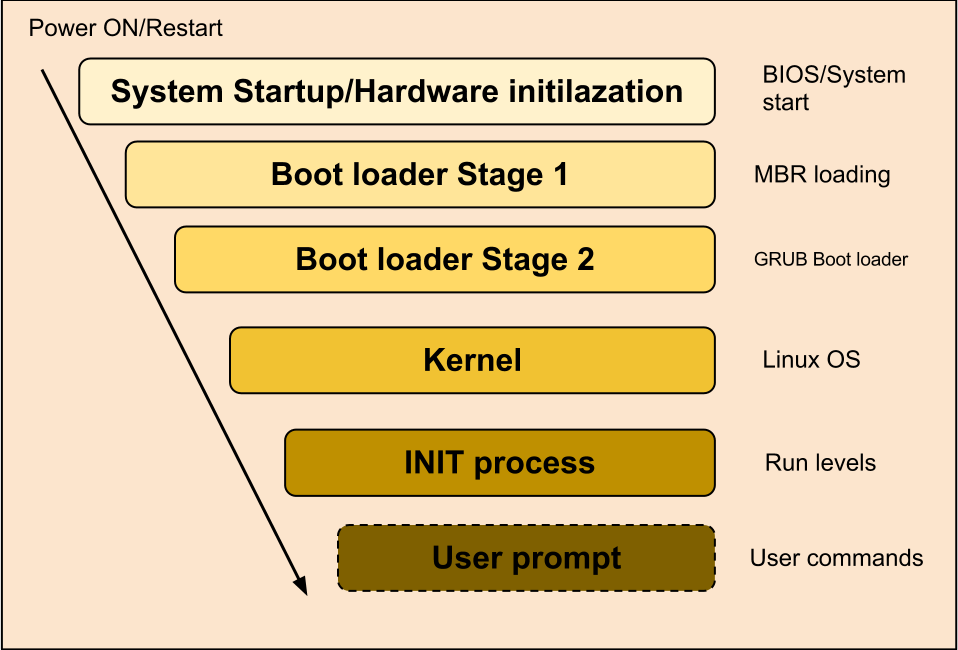
\includegraphics[scale=0.25]{img/Linux-Booting-process}
\end{center}

The getty process initiates login command and gives users with "login:" prompt, user should enter login name and password. The getty checks user credentials by verifying it with /etc/passwd and /etc/shadow files. If the credentials are ok, then it runs the configured shell (\$SHELL) in \$HOME configuration file (/etc/profile).

\begin{lstlisting}[caption=passwd and shadow files]
/etc/passwd
janague:x:1000:1000:janague,,,:/home/janague:/bin/bash

/etc/shadow
janague:$6$9MPUU0sm$M9jOGES..9pck2Yd4JucP9.sJad8WzA4XhI
\end{lstlisting}

There is an interesting debate going on about GUI (Graphical User Interface) and command-line shell, two modes for users to interact with the computer. Shell gives users more control and options, it also faster combination of keys are much faster than all that clicking, scrolling, and so on. Shells consume less resources (CPU and RAM). But in my opinion, the most important features of shells is that you can group and automate process in easy way.

\subsection{Shells}
Unix shell is simply a program that is used to start other programs, it is an essential component for all operating systems. Unix shell uses command in line and should be entered with a particular syntax.  Therefore, command-line shells also provide certain built-in features to the user, for example, cd is a program that you can execute in a shell and there are features like redirection to a file (ls $>$ file). Another facility in a shell is to read its commands from a text file, then the syntax and features may be thought of as a programming language, and such files are called \emph{scripts}.

There are a variety of UNIX shells to choose from, the original and most widely supported is called \emph{Bourne shell}. Its program filename is \emph{sh}. This shell do not offers many friendly features, for this reason, other shells were development, such as Korn shell (ksh), Bourne-again shell, zsh, and others. All these shells are supposed to be Bourne-compatible. In an effort to offer more power to shell programmers, another shell was developed in which the programming language was more closely related to the powerful "C" programming language. This shell was called the \emph{C-shell} (csh). It is more complex to use. There are other derived from C-shell, such as tcsh. And these are incompatible with Bourne-shells.

\subsubsection{Thompson shell}
The Thompson shell was the first Unix shell, introduced in the first version of Unix in 1971, and was written by Ken Thompson. It was not possible to use variables and scripting. It has some interesting features as a compact syntax for input/output redirection ($command1 >command2$), and the concept of pipes ($command1 | command2$), the output of one command could be passed to the input of another command, even they have been adopted by most other Unix shells.
\subsubsection{Bourne shell (sh)}
The Bourne shell was the default Unix shell of Unix Version 7, and most Unix-like systems continue to have /bin/sh. It was developed by Stephen Bourne at Bell Labs in 1977, it was a replacement for the Thompson shell in the Version 7 Unix. It provides output redirection, pipelines, variables, environment variables, flow control constructs (for, case, if), scopes, command substitution, invoking scripts using their filename, and other features. The Bourne shell was once standard on all branded Unix systems.

On the other hand, it was criticized because it was not properly programmed, and has not history and aliases features.
\subsubsection{C shell (csh)}
The C shell is a Unix shell that was created by Bill Joy while he was a graduate student at University of California, Berkeley in the late 1970s. It used in the BSD Unix system. The main design aims were that it should look more like the C programming language and independent of the platform (no only UNIX).

The C shell can also read commands from a file, called a script. Like all Unix shells, it supports command history, aliases, completing commands, filename wildcarding, piping, here documents, command substitution, variables and control structures for condition-testing and iteration.
On the other hand, it was not possible to use of functions.

\begin{center}
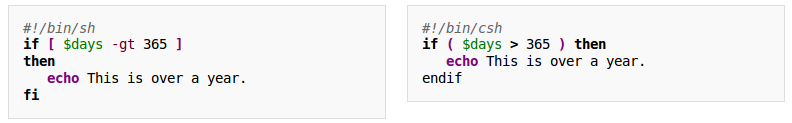
\includegraphics[scale=0.4]{img/sh_vs_csh}
\end{center}

\subsubsection{Tenex C shell (tcsh)}
Tcsh is an enhanced, but completely compatible version of the Berkeley UNIX C shell (csh), it was created by Ken Green in the Universidad Carnegie Mellon. The “t” in tcsh comes from the “T” in TENEX, which is an operating system of PDP-10. It was based on C programming language with improvements, such as completion, history, etc. Nowadays, the tcsh is the default root shell of FreeBSD, DragonFly BSD, and DesktopBSD. 

It includes a command-line editor, programmable word completion, spelling correction, a history mechanism, job control and a C-like syntax.  

\subsubsection{Korn shell (ksh)}
The Korn shell language was designed and developed by David G. Korn at AT\&T Bell Laboratories in 1983. ksh is intended to conform to the Shell Language Standard developed by the IEEE POSIX 1003.2 Shell and Utilities Language Committee. KornShell is backward-compatible with the Bourne shell and includes many features of the C shell. 
Until 2000, Korn shell remained AT\&T's proprietary software, therefore a number of free and open source alternatives were created, these include the public domain version, pdksh (openBSD), mksh (Android), GNU bash, and zsh. Since then it has been open source software, originally under a license particular to AT\&T, but in early 2005, it has been licensed under the Common Public License. 

The major features of the Korn shell are improved performance, Bourne shell compatibility, command-line editing, command history, enhanced I/O facilities, data types and attributes, integer arithmetic support, arrays, string, regular expressions, job control, aliases, variables, functions, directory navigation, enhanced debugging, and others.

\subsubsection{Bourne-again shell (bash)}
Bash is a Unix shell written by Brian Fox in 1989 for the GNU Project as a free software replacement for the Bourne shell (sh). It is a complete implementation of the IEEE Portable Operating System Interface for Unix (POSIX) and Open Group shell specification (IEEE POSIX P1003.2/ISO 9945.2). Bash is an sh-compatible shell that incorporates useful features from the Korn shell (ksh) and C shell (csh). Bash is free software and licenses as GPL v3.

The major features of the bash shell are command line editing and completion, unlimited size command history and re-entry, job Control, shell functions and aliases, default arguments, indexed arrays of unlimited size, integer arithmetic in any base from two to sixty-four, expansion (tilde, brace), substring, help, security, internationalization, command timing, and others.

\subsubsection{Z shell (zsh)}
The first version of zsh was written by Paul Falstad in 1990 when he was a student at Princeton University. The name zsh derives from Yale professor Zhong Shao's (then a teaching assistant at Princeton University). Zsh is a shell designed for interactive use, although it is also a powerful scripting language. 

The major features of the Z shell are command-line completion, command history, file globbing, variables, array, \emph{spelling correction}, \emph{fully customizable}, and many of the useful features of bash, ksh, and tcsh.
\subsection{Exercises}

\begin{lstlisting}[caption=Install csh shell]
janague@gon:~$ sudo apt-get install csh
Reading package lists... Done
Building dependency tree       
Reading state information... Done
The following NEW packages will be installed
  csh
0 upgraded, 1 newly installed, 0 to remove and 24 not 
upgraded.
Need to get 243 kB of archives.
After this operation, 406 kB of additional disk space 
will be used.
Get:1 http://gb.archive.ubuntu.com/ubuntu/ saucy/universe 
csh amd64 20110502-2ubuntu1 [243 kB]
Fetched 243 kB in 0s (376 kB/s)
Selecting previously unselected package csh.
(Reading database ... 562515 files and directories currently 
installed.)
Unpacking csh (from .../csh_20110502-2ubuntu1_amd64.deb) ...
Processing triggers for doc-base ...
Processing 1 added doc-base file...
Registering documents with scrollkeeper...
Processing triggers for man-db ...
Setting up csh (20110502-2ubuntu1) ...
update-alternatives: using /bin/bsd-csh to provide /bin/csh 
(csh) in auto mode
\end{lstlisting}

\begin{lstlisting}[caption=csh shell job control]
janague@gon:~$ csh
% set j = 1
% foreach n ( 1 2 3 4 5 )
?  echo "Welcome $j times"
? @ j++
? end
Welcome 1 times
Welcome 2 times
Welcome 3 times
Welcome 4 times
Welcome 5 times
\end{lstlisting}


\begin{lstlisting}[caption=Install pdksh shell]
janague@gon:~$ sudo apt-get install pdksh
Reading package lists... Done
Building dependency tree       
Reading state information... Done
The following extra packages will be installed:
  mksh
The following NEW packages will be installed
  mksh pdksh
0 upgraded, 2 newly installed, 0 to remove and 24 not 
upgraded.
Need to get 481 kB of archives.
After this operation, 901 kB of additional disk space 
will be used.
Do you want to continue [Y/n]? Y
Get:1 http://gb.archive.ubuntu.com/ubuntu/ saucy/main 
mksh amd64 46-2ubuntu1 [479 kB]
Get:2 http://gb.archive.ubuntu.com/ubuntu/ saucy/main
 pdksh all 46-2ubuntu1 [2,872 B]
Fetched 481 kB in 0s (557 kB/s)   
Selecting previously unselected package mksh.
(Reading database ... 562524 files and directories 
currently installed.)
Unpacking mksh (from .../mksh_46-2ubuntu1_amd64.deb) ...
Selecting previously unselected package pdksh.
Unpacking pdksh (from .../pdksh_46-2ubuntu1_all.deb) ...
Processing triggers for man-db ...
Setting up mksh (46-2ubuntu1) ...
update-alternatives: using /bin/mksh to provide /bin/ksh 
(ksh) in auto mode
Setting up pdksh (46-2ubuntu1) ...
\end{lstlisting}

\begin{lstlisting}[caption=pdksh shell job control]
janague@gon:~$ pdksh
$ j=1
$ for n in 1 2 3 4 5
> do
> echo "Welcome $j times"
> let j++
> done
Welcome 1 times
Welcome 2 times
Welcome 3 times
Welcome 4 times
Welcome 5 times

\end{lstlisting}

\subsection{Scripting}
Some of the files on a UNIX system are executable, called program. Some of these programs are compiled from source code, and these programs are sometimes known as binary executable. Others are not compiled, and only contain text, which are called scripts. There are many different \emph{interpreters} for these scripts, such as \emph{awk}, \emph{sed}, \emph{perl}, and others. The Bourne shell is simply one such interpreter.

Script could be a text file that contains the names of other UNIX programs in sequence, any UNIX command may be added to a script, such as:
\begin{lstlisting}
	pwd
	ls -C
	ate
\end{lstlisting}
The text file could make a file executable using chmod program or execute using shell program. $chmod +x scriptFile$. To run the file as a program simply type $./scriptFile$. If the directory that contains the scripts is in the PATH shell variable "./" is not require.

There are a basic usable commands to build script, such as: 
\begin{itemize}
	\item \emph{echo}: Its function is(to simple write its arguments in the standard output, and it is mainly used to display messages to the users of the script.
	\item \emph{read}: It is a shell built-in command for reading from standard input and storing the information in shell \emph{variables}. It is usually used to receive information to the user. Read command can break information of the line in several variables, using read command with variables separated by spaces or tabs.
	\item $>$ redirects output to a file and $>>$ appends to a file. $2>$ to redirect standard error.
	\item $|$ can be piped output to the input of any other program.
	\item Standard input can be read from any file using $<$.
	\item A command can be run asynchronously by using $\&$.
	\item $\#$ character is used to comments, and it is strongly encouraged to comment all the code.
\end{itemize}
There are four ways to run a shell script on the command-line:
\begin{enumerate}
	\item Using chmod program to make file executable.
	\item sh scriptfile
	\item . scriptfile     (The command uses the current shell)
	\item exec scriptfile  (Create a new shell and close when script has finished)
\end{enumerate}
To enable the shell to know what program should be run to interpret the script, the script interpreter can be specified on the first line of the script, in the following manner.
\begin{lstlisting}
	#!/bin/csh
\end{lstlisting}
\newpage

%------------------------------------------------------------------------------
% 6. Free Software hypervisors: A way to virtualization environments
\section{Free Software hypervisors}

\subsection{Introduction}
Virtualization, in computing, refers to the act of creating a virtual (rather than actual) version of something, including but not limited to a virtual computer hardware platform, operating system (OS), storage device, or computer network resources.

With virtualization you can separate operating system from hardware. This allows to consolidate a several physical servers in only one server using virtualization.

It is important to note that virtualization is not the same of cloud computing, which is a large concept and virtualization is a component of cloud computing.

\subsection{Hypervisors}
Hypervisor is a piece of software that allows installing several operating systems instances in the actual hardware (\emph{host}) [one physical server] at the same time. Those OS are called \emph{guests}. Each guests are isolated to others and has its own resources.

There are two types of hypervisors:
\begin{itemize}
	\item Type-1 Bare metal: hypervisor runs directly on the bare hardware.
	
	\begin{center}
		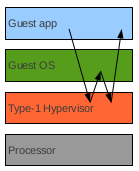
\includegraphics[scale=0.7]{img/type1}
	\end{center}
	
	Management Software usually installed on a different computer to manage all OS instances.
	Some business case are base on hypervisor free software and you pay for the Management software.  Besides, over allocation allows you to allocate more total resources to the instances of the operating systems then the physical server has. At any one time all Instances cannot use more resources then the total amount that the server has.
	\item Type-2 Hosted hypervisor: hypervisor runs as normal app on top of the host operating system. 
		
	\begin{center}
		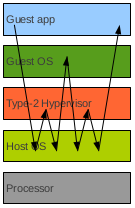
\includegraphics[scale=0.7]{img/type2}
	\end{center}
	
	In this case you do not need management software, because it is included in hosting operating system. 
	
\end{itemize}

These classification is not always clear cut, for example, Kernel-based Virtual Machine (KVM) is implemented as a kernel module for Linux which, when loaded, allows its host operating system to act as a bare metal (i.e., Type 1) hypervisor.However, as Linux distributions is operating system in their own right, one can argue that KVM is Type 2 hypervisors.

Different types of hardware virtualization include:
\begin{itemize}
    \item \emph{Full virtualization}: Almost complete simulation of the actual hardware to allow software, which typically consists of a guest operating system, to run unmodified.
    \item \emph{Partial virtualization}: Some but not all of the target environment is simulated. Some guest programs, therefore, may need modifications to run in this virtual environment.
    \item \emph{Paravirtualization}: A hardware environment is not simulated; however, the guest programs are executed in their own isolated domains, as if they are running on a separate system. Guest programs need to be specifically modified to run in this environment.
\end{itemize}

\subsection{Hypervisor products}
There are at least the following free software hypervisor products:
\begin{itemize}
	\item \emph{Xen}: It is a hypervisor using a microkernel design, The University of Cambridge Computer Laboratory developed the first versions of Xen. Its license is GNU General Public License (GPL), version 2. It is a type-1 hypervisor.
	
	Responsibilities of the hypervisor include memory management and CPU scheduling of all virtual machines ("domains"), and for launching the most privileged domain ("dom0") - the only virtual machine which by default has direct access to hardware. From the dom0 the hypervisor can be managed and unprivileged domains ("domU") can be launched.
	
	Xen allows paravirtualization and full virtualization.
	\item \emph{KVM}: KVM (for Kernel-based Virtual Machine) is a full virtualization solution for Linux on x86 hardware containing virtualization extensions (Intel VT or AMD-V). It consists of a loadable kernel module, kvm.ko, that provides the core virtualization infrastructure and a processor specific module, kvm-intel.ko or kvm-amd.ko. KVM also requires a modified QEMU although work is underway to get the required changes upstream. It is a type-1 hypervisor.
	\item \emph{VirtualBox}: It is a powerful x86 and AMD64/Intel64 virtualization product. Not only is VirtualBox an extremely feature rich, high performance product for enterprise customers, it is freely available as Open Source Software under the terms of the GNU General Public License (GPL), version 2. It is a type-2 hypervisor. It also requires QEMU to emulate some virtual devices, and it uses a recompiler of QEMU as fallback mechanism.
\end{itemize}

\newpage
\subsection{OpenStack}
OpenStack is a cloud operating system that controls large pools of compute, storage, and networking resources throughout a datacenter, all managed through a dashboard that gives administrators control while empowering their users to provision resources through a web interface. Its license is Apache license, and developed in Python.

	\begin{center}
		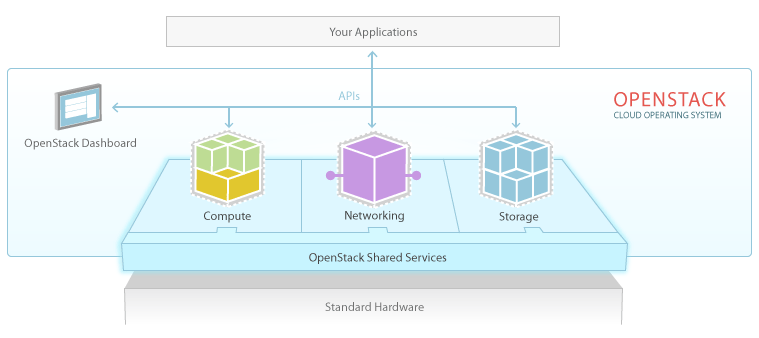
\includegraphics[scale=0.5]{img/openStack}
	\end{center}

\begin{itemize}
	\item \emph{Compute (Nova)}: Provision and manage large networks of virtual machines.
	\item \emph{Storage (Swift)}: Object and Block storage for use with servers and applications.
	\item \emph{networking}: Pluggable, scalable, API-driven network and IP management
	\item \emph{Dashboard (Horizon)}: Graphical interface to access, provision and automate cloud-based resources.
	\item \emph{Shared services}: Spanning the three pillars of compute, storage and networking, making it easier to implement and operate your cloud.
\end{itemize}

\newpage

\bibliographystyle{abbrv}
\bibliography{caseStudiesIReport}

 \nocite{*}

\end{document}